\section{THERMR}
\label{sTHERMR}

\hypertarget{sTHERMRhy}{The}
THERMR\index{THERMR|textbf} module generates pointwise neutron
scattering cross sections in the thermal energy range
\index{thermal cross sections} and adds them to an existing
PENDF\index{PENDF} file.  The cross sections can then be
group-averaged, plotted, or reformatted in subsequent modules.
THERMR works with either the original ENDF/B-III thermal
format\cite{old102} and data files\cite{GAreport} (which were
also used for ENDF/B-IV and -V), or the newer ENDF-6
format\cite{ENDF102}.  Coherent elastic\index{coherent elastic}
cross sections are generated for crystalline materials using
either parameters given in an ENDF-6 format evaluation or an extended
version of the method of HEXSCAT\cite{HEXSCAT}\index{HEXSCAT}.
Incoherent elastic\index{incoherent elastic} cross sections
for non-crystalline materials such as polyethylene and ZrH
can be generated either from parameters in an ENDF-6 format file or by
direct evaluation using parameters included in the THERMR coding.
Inelastic\index{thermal inelastic} cross sections and
energy-to-energy transfer matrices can be produced for a gas
of free atoms, or for bound scatterers when ENDF
$S(\alpha,\beta)$\index{$S(\alpha,\beta)$} scattering functions
are available.  This function has previously been performed
using FLANGE-II\cite{FLANGE}\index{FLANGE-II}.  THERMR has the
following features:

\begin{itemize}
\begin{singlespace}
\item The energy grid for coherent elastic scattering is produced
   adaptively so as to represent the cross section between the
   sharp Bragg edges to a specified tolerance using linear interpolation.

\item The secondary energy grid for inelastic incoherent scattering
   when using $E$-$E'$-$\mu$ ordering is produced adaptively so as to
   represent all structure with linear interpolation.  Discrete-angle
   representations are used to avoid the limitations of Legendre
   expansions.

\item An option to use $E$-$\mu$-$E'$ ordering is available.  Dependences
   on $\mu$ and $E'$ are constructed adaptively.

\item Incoherent cross sections are computed by integrating the
   incoherent distributions for consistency.

\item Free-atom incoherent scattering is normalized to the Doppler
   broadened elastic scattering cross section in order to provide an
   approximate representation of resonance scattering and to preserve
   the correct total cross section.

\item Hard-to-find parameters for the ENDF/B-III evaluations are included
   in the code for the user's convenience.

\item ENDF-6 format files can be processed.  This gives the evaluator
   more control over the final results, because all parameters
   needed to compute the cross sections are contained in the file.
\end{singlespace}
\end{itemize}

This chapter describes the THERMR module in NJOY2016.0.

\subsection{Coherent Elastic Scattering}
\label{ssTHERMR_coh}

In crystalline solids consisting of coherent scatters --- for example,
graphite --- the so-called ``zero-phonon term'' leads to interference
scattering from the various planes of atoms of the crystals making up
the solid.  There is no energy loss in such scattering, and the ENDF
term for the reaction is coherent elastic scattering.
\index{coherent elastic} The cross section may be represented
as follows:

\begin{equation}
   \sigma^{\rm coh}(E,E',\mu)=\frac{\sigma_c}{E}
     \sum_{E_i>E} f_i\,{\rm e}^{-2WE_i}\,\delta(\mu-\mu_0)
      \,\delta(E-E')\,\,,
\label{coh}
\end{equation}

\noindent
where

\begin{equation}
   \mu_0=1-2\frac{E_i}{E}\,\,,
\end{equation}

\noindent
and the integrated cross section is given by

\begin{equation}
   \sigma^{\rm coh}=\frac{\sigma_c}{E}
      \sum_{E_i>E}\,f_i\,{\rm e}^{-2WE_i}\,\,.
\label{cohxs}
\end{equation}

\noindent
In these equations, $E$ is the incident neutron energy, $E'$ is the
secondary neutron energy, $\mu$ is the scattering cosine in the
laboratory (LAB) reference system, $\sigma_c$ is the characteristic
coherent cross section\index{coherent cross section} for the material,
$W$ is the effective Debye-Waller coefficient\index{Debye-Waller factor}
(which is a function of temperature), the $E_i$ are the so-called
``Bragg edges'', \index{Bragg edges} and the $f_i$ are related to
the crystallographic structure factors.

It can be seen from Eq.~\ref{cohxs} and the example in Fig.~\ref{cohfig}
that the coherent elastic cross section is zero before the first Bragg edge,
$E_1$ (typically about 2 to 5 meV).  It then jumps sharply to a value
determined by $f_1$ and the Debye-Waller term.  At higher energies, the
cross section drops off as $1/E$ until $E{=}E_2$.  It then takes another
jump and resumes its $1/E$ drop-off.  The sizes of the steps in the cross
section gradually get smaller, and at high energies there is nothing left
but an asymptotic $1/E$ decrease (typically above 1 to 2 eV).

\begin{figure}[thb]\centering
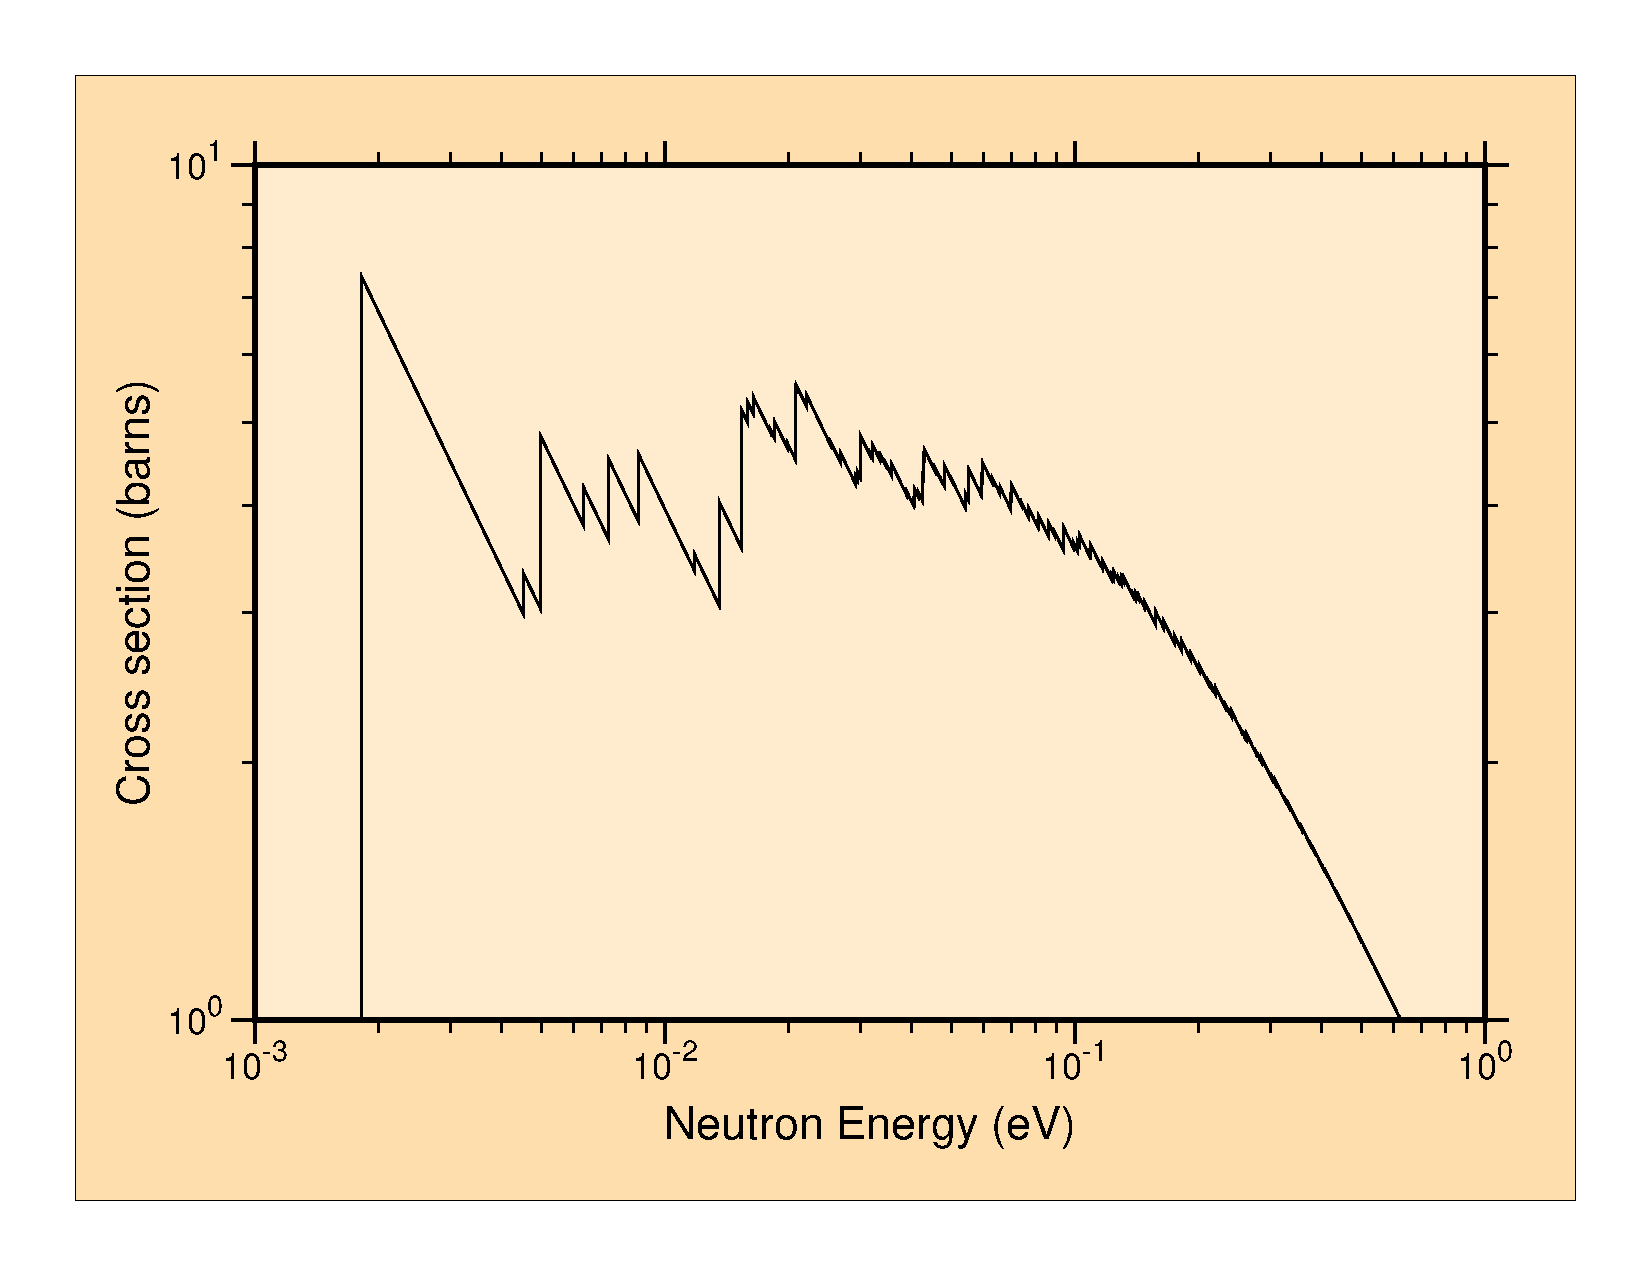
\includegraphics[keepaspectratio,height=3.5in, angle=0]{figs/thermr1ack}
\caption[Example of coherent elastic cross section for a crystalline
material (graphite)]
 {Typical behavior of the coherent elastic scattering cross section for a
 crystalline material as computed by THERMR. This cross section is for
 graphite at 293.6K.}
\label{cohfig}
\end{figure}

For evaluations in the ENDF-6 format, the section MF=7/MT=2 contains
the quantity $E\sigma^{\rm coh}(E)$ as a function of energy and
temperature. The energy dependence is given as a histogram with breaks
at the Bragg energies.  The cross section is easily recovered from this
representation by dividing by $E$.  The $E_i$ are easily found as the
tabulation points of the function, and the $f_i$ for a point can be
obtained by subtracting the value at the previous point.

For evaluations using the older ENDF/B-III thermal format, it is
necessary to compute the $E_i$ and $f_i$ in THERMR.  The methods used
are based on HEXSCAT\index{HEXSCAT} and work only for the hexagonal
materials graphite, Be, and BeO.  The Bragg edges are given by

\begin{equation}
   E_i=\frac{\hbar^2\tau_i^2}{8m}\,\,,
\end{equation}

\noindent
where $\tau_i$ is the length of the vectors of one particular
``shell'' of the reciprocal lattice, and $m$ is the neutron mass.
The $f_i$ factors are given by

\begin{equation}
   f_i=\frac{\pi^2\hbar^2}{2mNV}\sum_{\rm shell}|F(\tau)|^2\,\,,
\end{equation}

\noindent
where the shell sum extends over all reciprocal lattice vectors
of the given length, $N$ is the number of atoms in the unit cell,
and  $F$ is the crystallographic structure factor.  The calculation
works by preparing a sorted list of precomputed $\tau_i$ and $f_i$
values.  As $\tau_i$ gets large, the values of $\tau_i$ get more and more
closely spaced.  In order to save storage and run time, a range of $\tau$
values can be lumped together to give a single effective $\tau_i$ and
$f_i$.  This device washes out the Bragg edges at high energies while
preserving the proper average cross section and angular dependence.
The current grouping factor is 5\% (see \cword{eps} in \cword{sigcoh}).

Lattice constants (given in \cword{sigcoh} for graphite, Be, and BeO), form
factor formulas (see \cword{form}), Debye-Waller coefficients, and methods
for computing reciprocal lattice vectors were borrowed directly
 from HEXSCAT.

The energy grid for $E$ is obtained adaptively (see \cword{coh}).  A panel
extending from just above one Bragg edge to just below the next
higher edge is subdivided by successive halving until linear
interpolation is within a specified fractional tolerance (\cword{tol}) of the
exact cross section at every point.  This procedure is repeated for
every panel from the first Bragg edge to the specified maximum
energy for the thermal treatment (\cword{emax}).

The code usually computes and writes out the cross section of
Eq.~\ref{cohxs}, the average over $\mu$ of Eq.~\ref{coh},
which is sometimes called the P$_0$ cross section.  Subsequent modules can
deduce the correct discrete scattering angles $\mu_0$ from the
location of the Bragg edges $E_i$ and the factors $f_i$ from the
cross section steps at the Bragg edges (see
\hyperlink{sGROUPRhy}{GROUPR}\index{GROUPR}).
Legendre cross sections can also be computed by making a small change
to the code.  It is not necessary to give the P$_1$, P$_2$, and P$_3$ cross
sections explicitly as was done in some earlier codes or in File 4
of the ENDF thermal tapes.

\subsection{Incoherent Inelastic Scattering}
\label{ssTHERMR_incoh_inel}

In ENDF/B notation, the thermal incoherent scattering cross section
\index{incoherent inelastic} is given by

\begin{equation}
   \sigma^{\rm inc}(E,E',\mu)=\frac{\sigma_b}{2kT}
    \sqrt{\frac{E'}{E}}\,{\rm e}^{-\beta/2}S(\alpha,\beta)\,\,,
\label{incoh}
\end{equation}

\noindent
where $E$ is the initial neutron energy, $E'$ is the energy of the
scattered neutron, $\mu$ is the scattering cosine in the laboratory
system, $\sigma_b$ is the characteristic bound incoherent cross
section for the nuclide, $T$ is the Kelvin temperature, $\beta$ is the
dimensionless energy transfer,

\begin{equation}
   \beta=\frac{E'-E}{kT}\,\,,
\label{ebeta}
\end{equation}

\noindent
$\alpha$ is the dimensionless momentum transfer,

\begin{equation}
   \alpha=\frac{E'+E-2\mu\sqrt{EE'}}{AkT}\,\,,
\end{equation}

\noindent
$k$ is Boltzmann's constant\index{Boltzmann constant}, and $A$
is the ratio of the scatter mass to the neutron mass.  The
bound scattering cross section\index{bound atom scattering cross section}
is usually given in terms of the characteristic free cross
section,\index{free atom scattering cross section} $\sigma_f$,

\begin{equation}
   \sigma_b=\sigma_f\frac{(A+1)^2}{A^2}\,\,.
\end{equation}

\noindent
The scattering law\index{scattering law}
$S(\alpha,\beta)$\index{$S(\alpha,\beta)$} describes the binding of the
scattering atom in a material.  For a free gas\index{free gas}
of scatterers with no internal structure

\begin{equation}
   S(\alpha,\beta)=\frac{1}{\sqrt{4\pi\alpha}}
    \exp\left\{-\frac{\alpha^2+\beta^2}{4\alpha}\right\}\,\,.
\label{free}
\end{equation}

\noindent
For binding in solids and liquids, $S(\alpha,\beta)$ for a number of
important moderator materials is available in ENDF/B File 7
\index{File 7} format.  The scattering law is given as tables of $S$
versus $\alpha$ for various values of $\beta$.  Values of
$S$ for other values of $\alpha$ and $\beta$ can be obtained by interpolation.
The scattering law is normally symmetric in $\beta$ and only has to be
tabulated for positive values, but for materials like orthohydrogen and
parahydrogen\index{ortho hydrogen}\index{para hydrogen}
of interest for cold moderators at neutron scattering facilities,
this is not true.  These kinds of materials are identified by the ENDF-6 LASYM
option, and THERMR assumes that the scattering law is given explicitly
for both positive and negative values of $\beta$.

If the $\alpha$ or $\beta$ required is outside the range of the table
in File 7, the differential scattering cross section can be computed
using the short collision time (SCT) approximation
\index{short collision time}

\begin{equation}
   \sigma^{\rm SCT}(E,E',\mu)=\frac{\sigma_b}{2kT}
     \frac{\sqrt{E'/E}}{\sqrt{4\pi\,\alpha\,T_{\rm eff}/T}}
      \exp\left\{-\frac{(\alpha-|\beta|)^2}{4\,\alpha}
        \frac{T}{T_{\rm eff}}-\frac{\beta+|\beta|}{2}\right\}\,\,,
\end{equation}

\noindent
where $T_{\rm eff}$ is the effective temperature for the SCT approximation.
These temperatures are available\cite{GAreport} for the older
ENDF/B-III evaluations; they are usually somewhat larger
than the corresponding Maxwellian temperature $T$.  For the convenience
of the user, the values of $T_{\rm eff}$ for the common moderators are
included as defaults (see input instructions).  For the newer ENDF-6
format, the effective temperatures are included in the data file.
However, there is a complication.  Some evaluations give $S(\alpha,\beta)$ for
a molecule or compound (in the ENDF/B-III files, these cases are
BeO and C$_6$H$_6$).  The corresponding SCT approximation must contain
terms for both atoms.  The two sets of bound cross sections and effective
temperatures are included in the data statements in THERMR, and they
can be given in the new ENDF-6 format if desired.

THERMR expects the requested temperature $T$ to be one of the temperatures
included on the ENDF/B thermal file, or within a few degrees of that
value (296K is used if 300K is requested).  Intermediate temperatures
should be obtained by interpolating between the resulting cross sections
and not by interpolating $S(\alpha,\beta)$.

The cross sections for incoherent inelastic scattering are computed
in the \cword{calcem}\index{calcem@{\ty calcem}} subroutine.  There
are two possible orderings of the basic variables allowed (see
\cword{iform}).  For $E$-$E'$-$\mu$ ordering, the secondary energy grid
for incoherent scattering is obtained adaptively.  A stack is first primed
with the point at zero and the first point above zero that can be derived
from the positive and negative values of $\beta$ from the evaluator's
$\beta$ grid using Eq.~\ref{ebeta}.  (For free-gas scattering, the
$\beta$ grid is taken to have nine entries between 0.0 eV and 25.0 eV).
This interval is then subdivided by successive halving until the
cross section obtained by linear interpolation is within the specified
tolerance of the correct cross section (from
\cword{sigl}\index{sigl@{\ty sigl}}). The next
highest energy derived from the $\beta$ grid is then calculated,
and the subdivision process is repeated for this new interval.
This process is continued until the $\beta$ grid has been exhausted.
Excess points with zero cross section are removed before writing
the spectrum into File 6.  This procedure is sure to pick up all the
structure in the evaluation; giving points related to the $\beta$
grid avoids excessive work in trying to fit sharp corners introduced by
breaks in the interpolation of $S(\alpha,\beta)$.  Fig.~\ref{graph}
shows how the procedure picks up features resulting from the sharp
excitation features in the graphite phonon frequency distribution.

\begin{figure}[thb]\centering
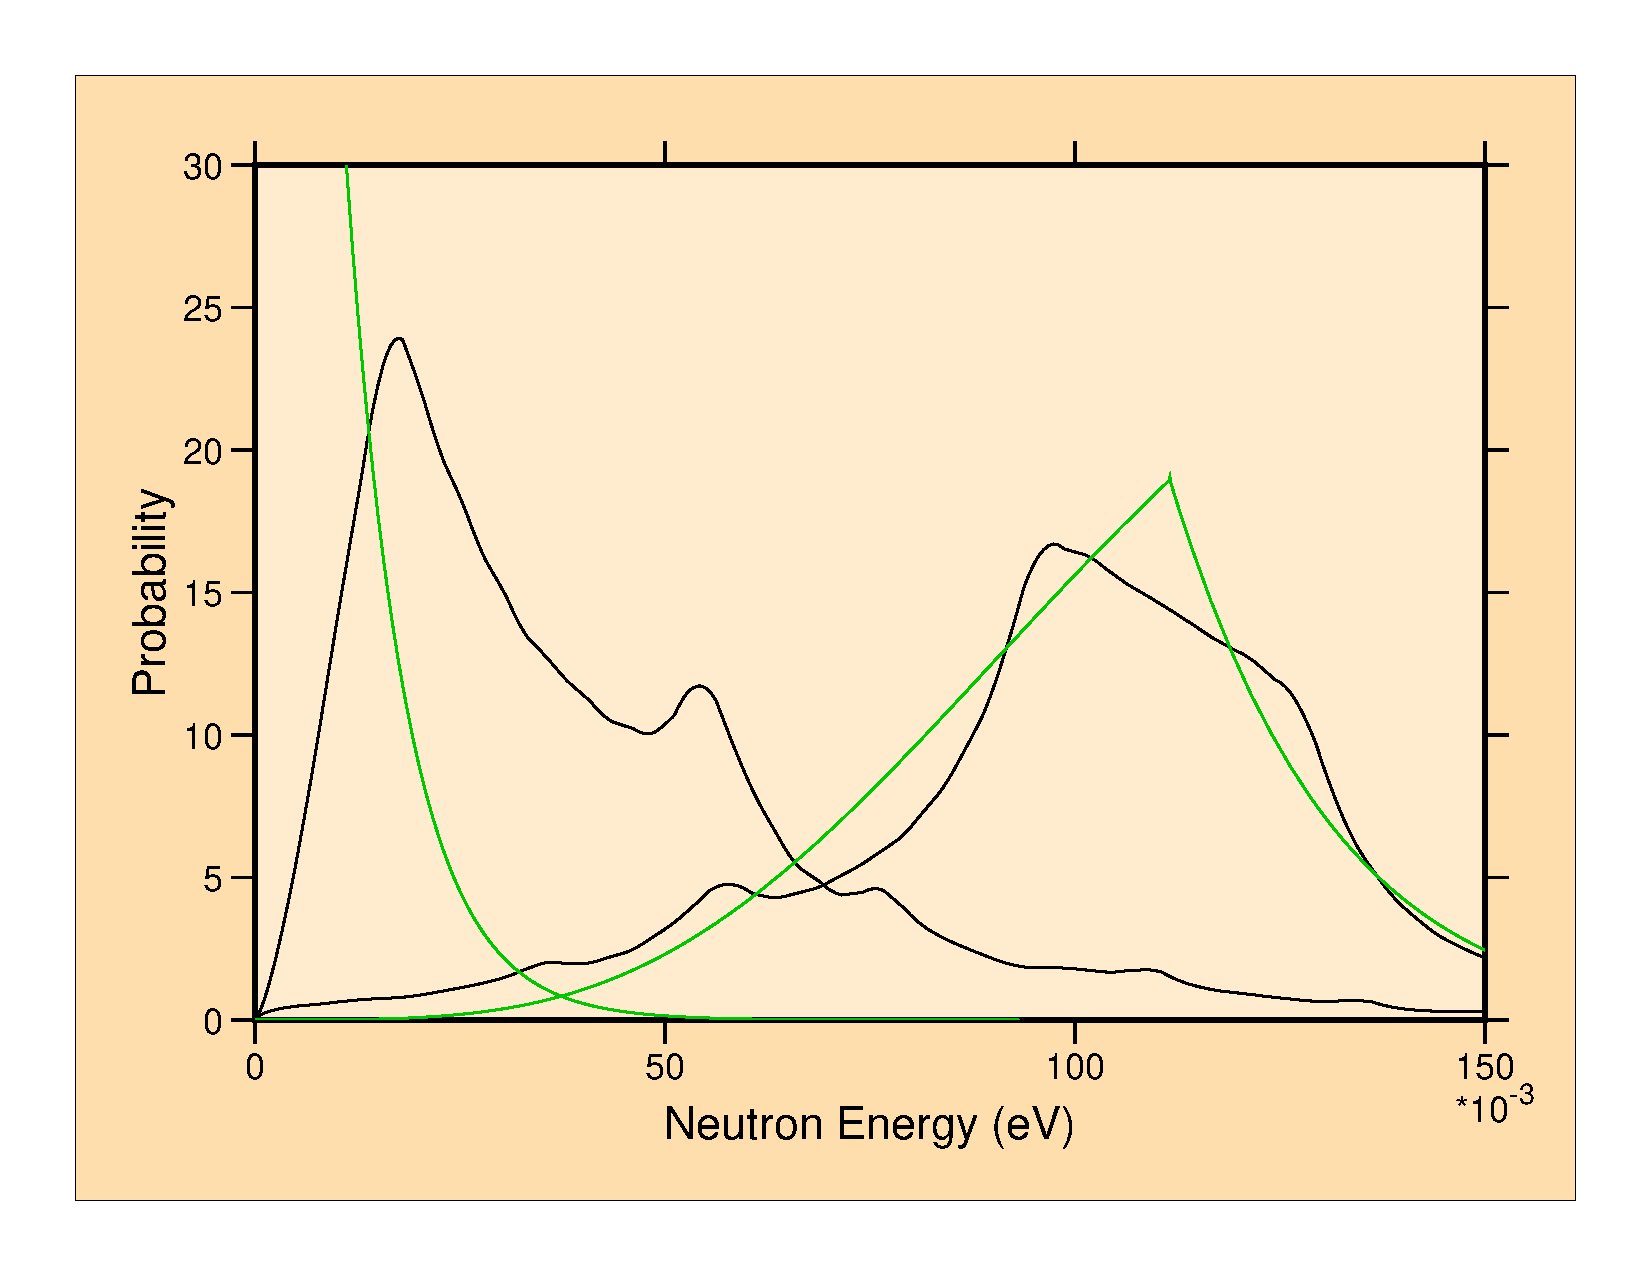
\includegraphics[keepaspectratio, height=3.0in, angle=0]{figs/thermr2ack}
  \caption[Adaptive reconstruction of emission spectra (graphite)]{Adaptive
 reconstruction of two of the emission curves for graphite at 293.6K
 (E=.00016 eV to the left, and E=.1116 eV to the right).  Note the
 presence of excitation features from the phonon frequency spectrum
 for both upscatter and downscatter.  The breaks in the curves are due
 to $\beta$ interpolation in $S(\alpha,\beta)$ and not to the tolerances
 in the reconstruction process.  The green curves are the corresponding
 free gas results.}
\label{graph}
\end{figure}

The result of this adaptive reconstruction is easily integrated by the
trapezoid rule to find the incoherent cross section at energy $E$.

The cross section for one particular $E{\rightarrow}E'$ is the integral
over the angular variable of Eq.~\ref{incoh}.  The angular dependence
is obtained by adaptively subdividing the cosine range until the actual
angular function (see \cword{sig}\index{sig@{\ty sig}}) is represented
by linear interpolation to within a specified tolerance.  The integral
under this curve is used in calculating the secondary-energy dependence
as described above.  Rather than providing the traditional Legendre
coefficients, THERMR divides the angular range into equally probable
cosine bins and then selects the single cosine in each bin that
preserves the average cosine in the bin.  These equally probable
cosines can be converted to Legendre coefficients easily
when producing group constants, and they are suitable for direct use in
Monte Carlo codes.  For strongly peaked functions, such as scattering for
$E{\gg}kT$ when the result begins to look ``elastic'', all the discrete
angles will be bunched together near the scattering angle defined by
ordinary kinematics.  This behavior cannot be obtained with ordinary
P$_3$ Legendre coefficients.  Conversely, if such angles are converted to
Legendre form, very high orders can be used.  If a direct calculation of
Legendre components is desired, reverse the sign of \cword{nnl} in
\cword{calcem}.

The incident energy grid\index{thermal energy grid} is currently stored
directly in the code (see \cword{egrid} in \cword{calcem}).  The choice
of grid for $\sigma^{\rm inc}(E)$ is not critical since the cross section
is a slowly varying function of $E$.  However, the energy grid
would seem to be important for the emission spectra.  In order
to demonstrate the problem, two perspective plots of
the full energy distribution of incoherent inelastic scattering from
graphite at 293.6K are shown in Figs.~\ref{dist} and \ref{dist2}.
The second plot is simply an expansion of the high-energy region
of the distribution.

\begin{figure}[thb]\centering
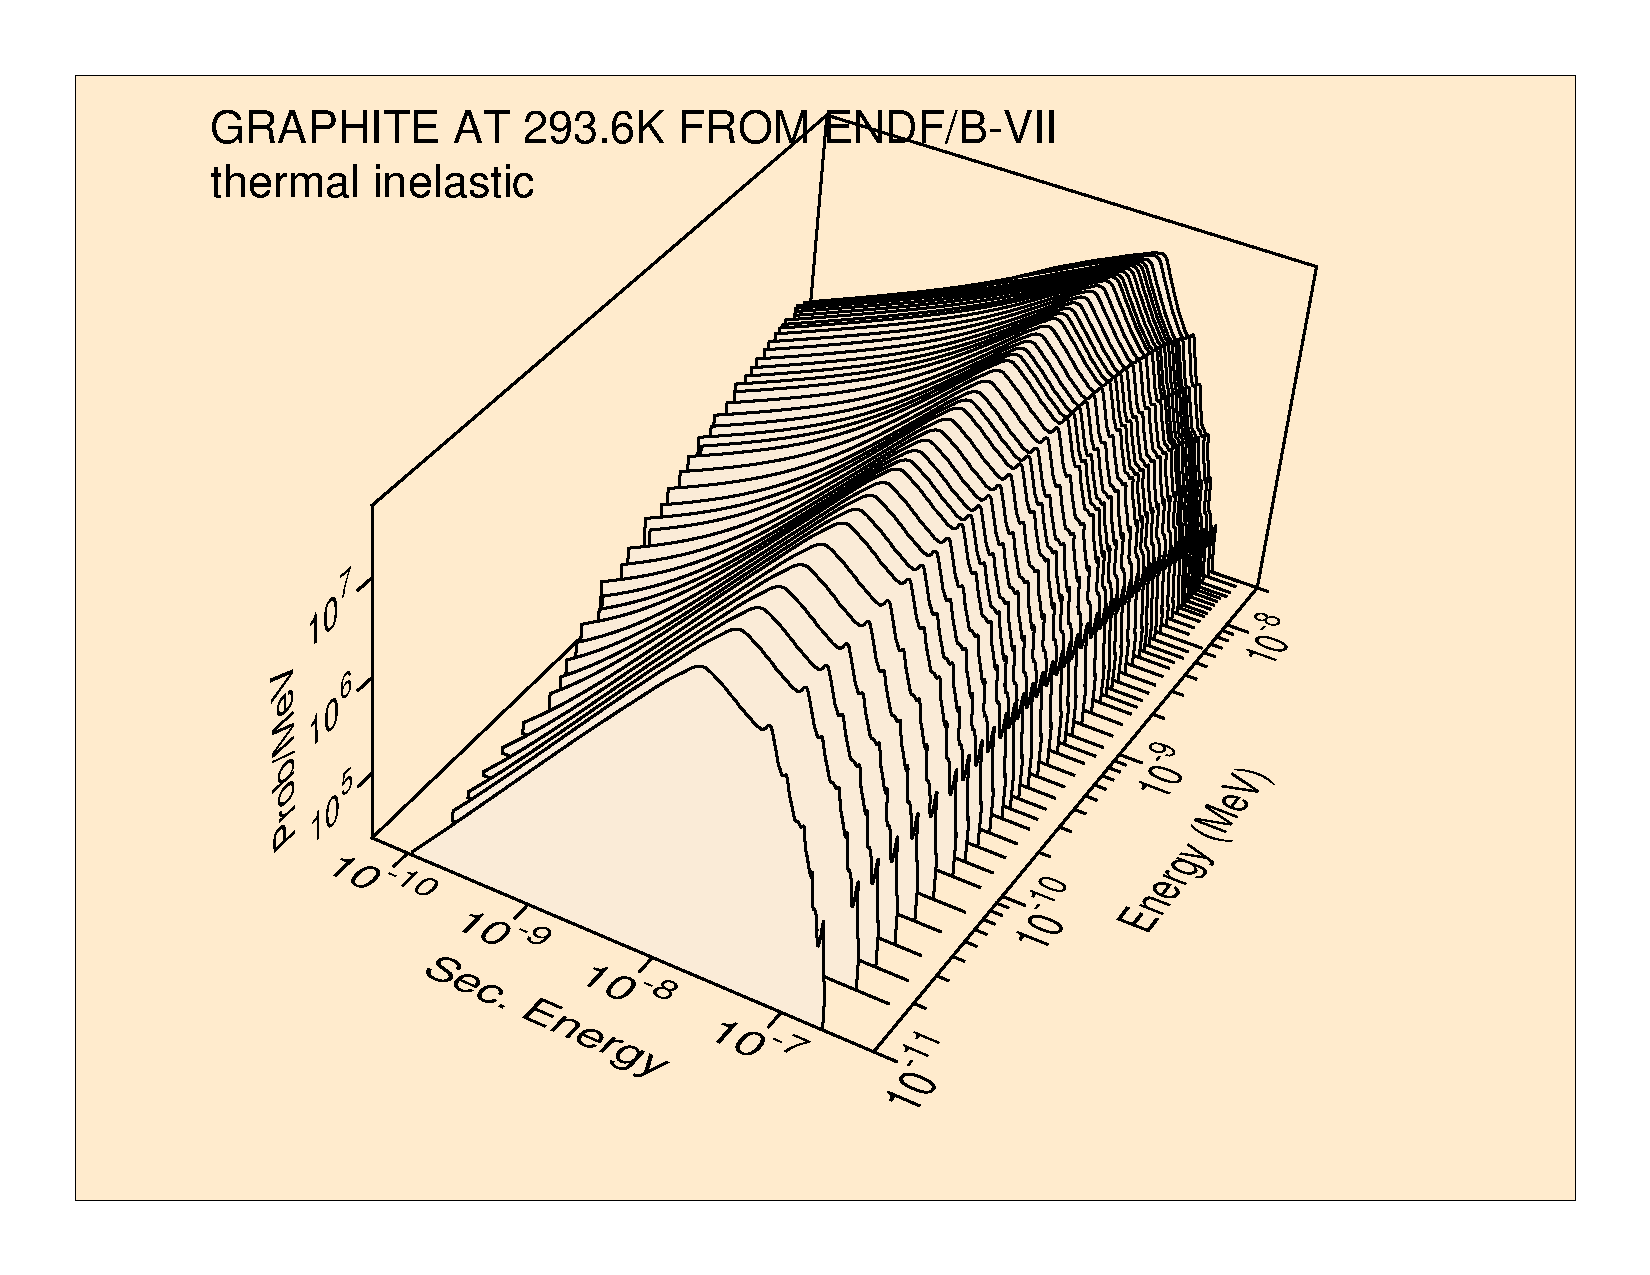
\includegraphics[keepaspectratio,height=3.0in, angle=0]{figs/thermr3ack}
\caption[Neutron distribution for incoherent inelastic scattering from graphite
 (T = 293.6K)]{Neutron distribution for incoherent inelastic scattering from
 graphite (T = 293.6K).}
\label{dist}
\end{figure}

\begin{figure}[thb]\centering
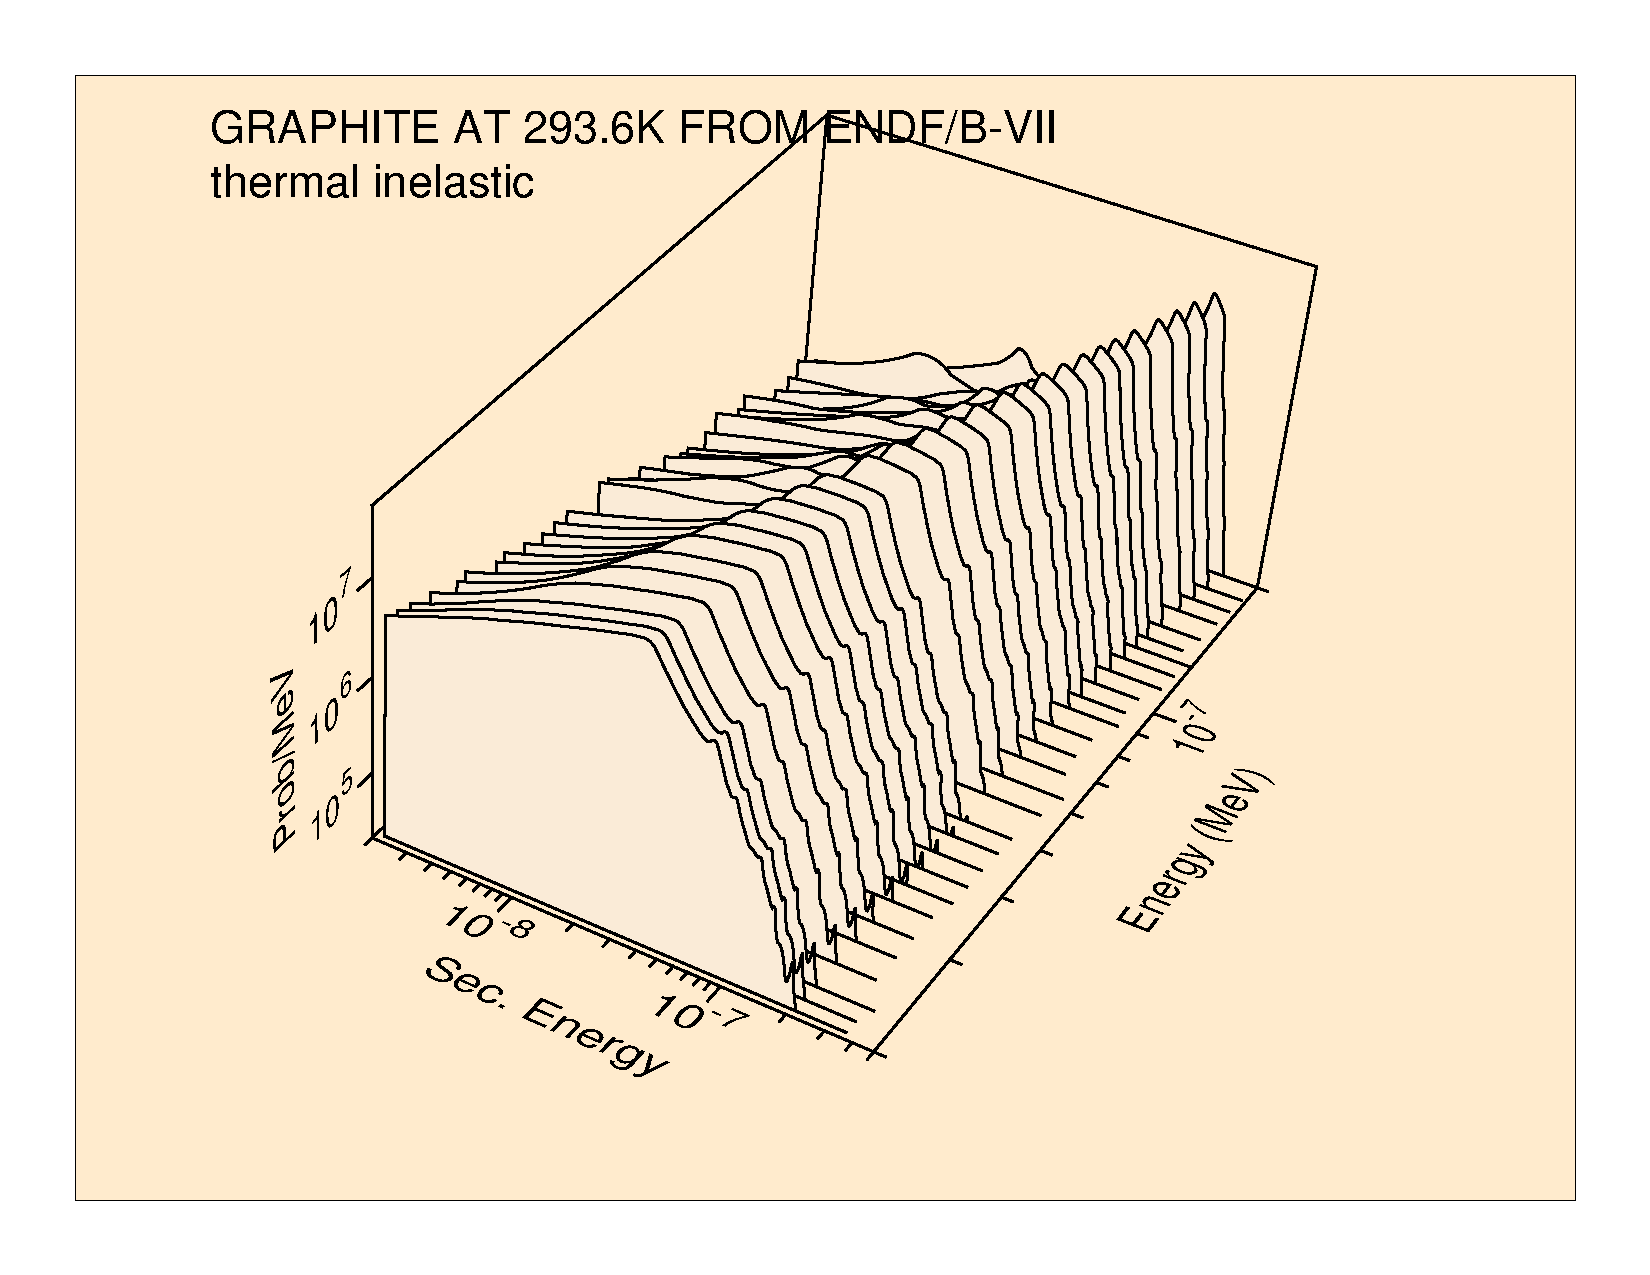
\includegraphics[keepaspectratio, height=3.0in, angle=0]{figs/thermr4ack}
  \caption[Neutron distribution for incoherent inelastic scattering
  from graphite
 (T = 293.6K), expanded view]{Expanded view of the high-energy region
 of the graphite incoherent inelastic distribution.}
\label{dist2}
\end{figure}

It is clear that $\sigma^{\rm inc}(E,E')$ for one value of $E'$ is
a very strongly energy-dependent function for the higher incident
energies.  However, as shown in Fig.~\ref{dist2}, the shape
of the secondary energy distribution changes more slowly,
with the peak tending to follow the line $E'{=}E$.  This behavior
implies that a relatively coarse incident energy grid might prove
adequate if a suitable method is used to interpolate between the
shapes at adjacent $E$ values.  One such interpolation scheme is
implemented in \hyperlink{sGROUPRhy}{GROUPR}\index{GROUPR}.  The
use of discrete angles is
especially suitable for this interpolation scheme.

Strictly speaking, the scattering law for free-gas scattering
given in Eq.~\ref{free} is only applicable to scatterers with no
internal structure.  However, many materials of interest in reactor
physics have strong scattering resonances in the thermal range
(for example, $^{240}$Pu and $^{135}$Xe).  The Doppler broadened elastic
cross section produced by BROADR\index{BROADR} is formally correct for
a gas of resonant scatterers, but the cross section resulting from
Eq.~\ref{free} is not.  In order to allow for  resonance scattering
in a way that at least provides the correct total cross section, THERMR
renormalizes the free-atom scattering to the broadened elastic cross
section.  The secondary energy distribution will still be incorrect.

The built-in grid for incident neutron energies is suitable for
normal temperatures found in reactors.  For higher temperatures
(higher than \cword{break}=3000), the grid values are scaled up
to span the kinds of energies expected.

If the $E$-$\mu$-$E'$ option is selected (\cword{iform}=1), an
adaptive reconstruction of the angular cross section
$\sigma(E,\mu)$ is performed.  For each $\mu$ value, the
secondary energy spectrum is generated adaptively, and the
integral over that spectrum is saved as $\sigma(E,\mu)$.
The results are written out using the ENDF-6 format
File 6/law 7 option.  This ordering is more like the results
of experiments, and the THERMR results can be used to compare
to experiment.  See Fig.~\ref{ang2} for a figure based on
this kind of ordering.

\begin{figure}[thb]\centering
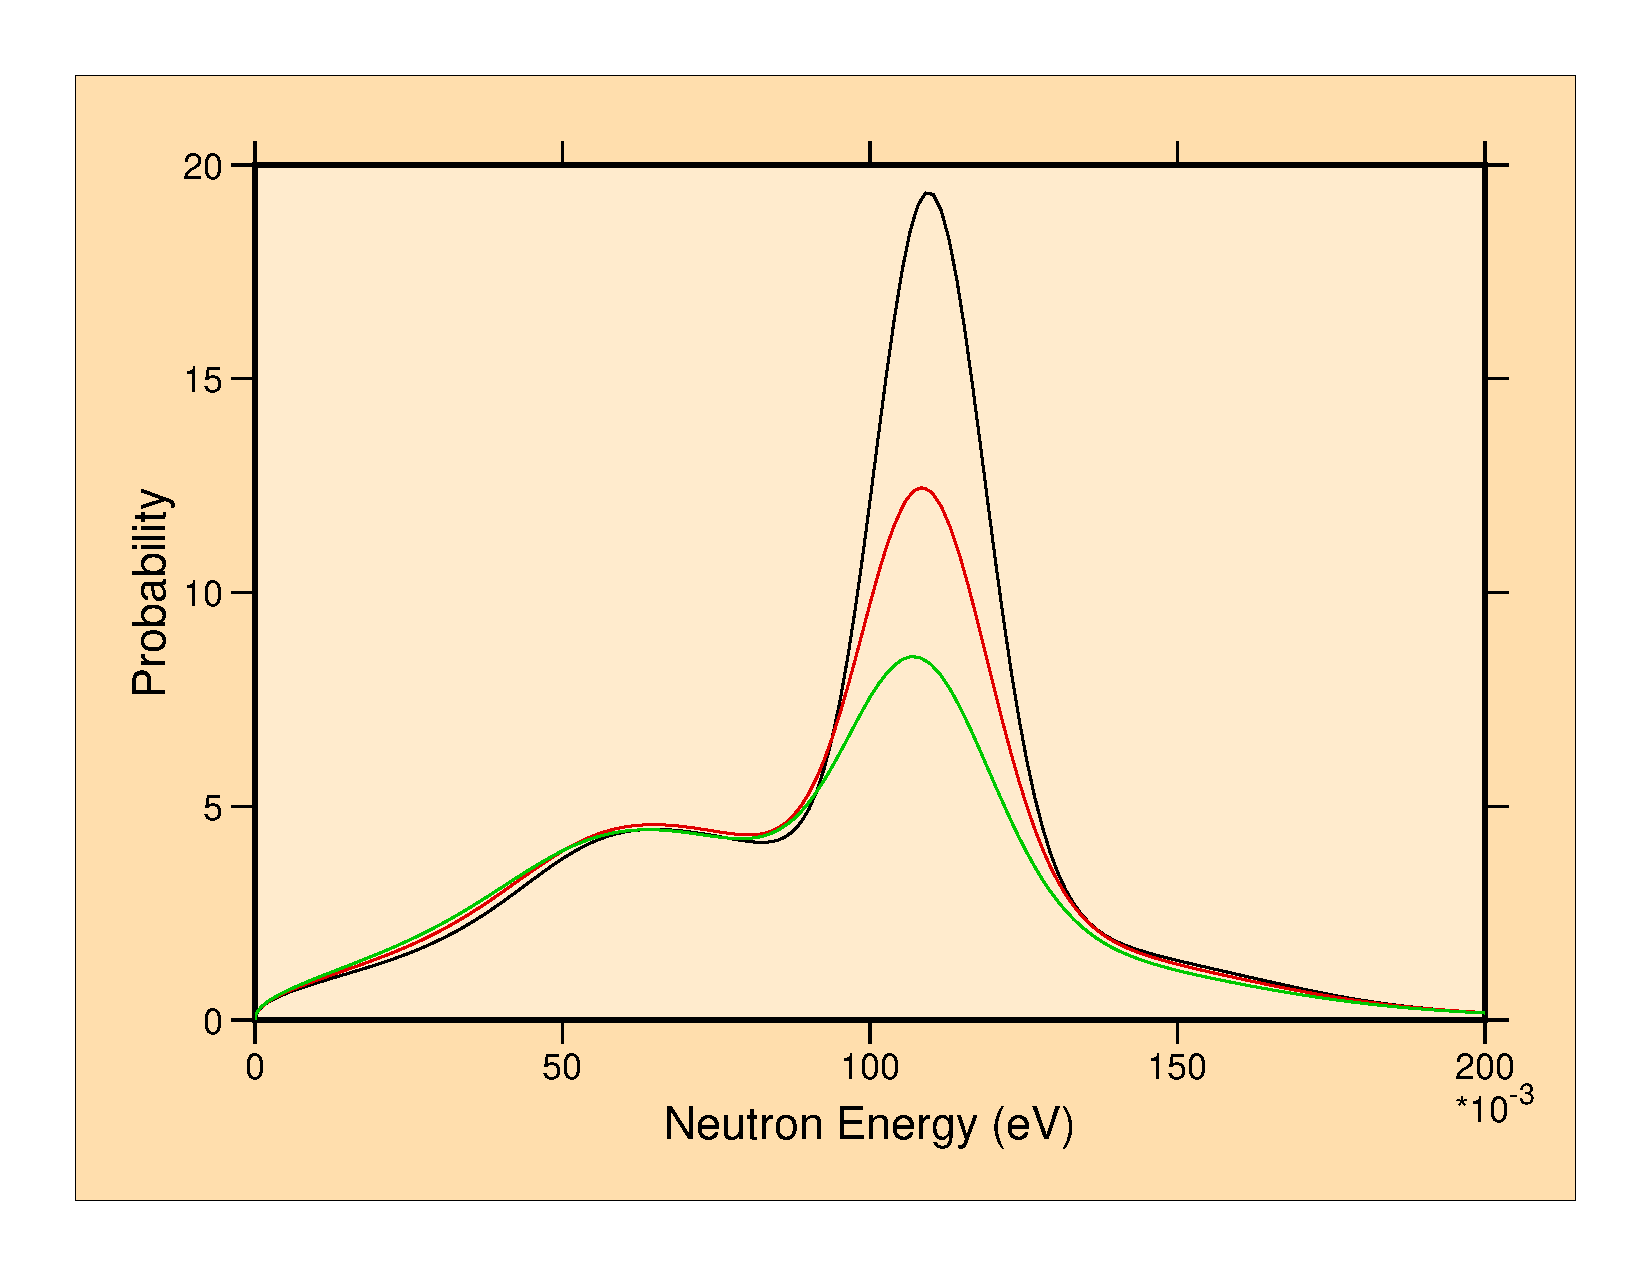
\includegraphics[keepaspectratio, height=3.5in, angle=0]{figs/thermr7ack}
\caption[Distributions for H in H$_2$O with $E$-$\mu$-$E'$ ordering]
{Example of distributions for H in H$_2$O with $E$-$\mu$-$E'$ ordering.  The
 incident energy is 0.115 eV.  The black curve is at 51.3 deg, the red
 curve is at 60 deg, and the green curve is at 68 deg.}
\label{ang2}
\end{figure}

\subsection{Incoherent Elastic Scattering}
\label{ssTHERMR_incoh_el}

In hydrogenous solids, there is an elastic (no energy loss) component
of scattering arising from the zero-phonon term that can be treated in
the incoherent approximation because of the large incoherent cross
section of hydrogen.  The ENDF term for this process is incoherent
elastic scattering\index{incoherent elastic}, and it is found in the
materials polyethylene and zirconium hydride.
\index{polyethylene}
\index{zirconium hydride}
The differential cross section is given by

\begin{equation}
   \sigma^{\rm iel}(E,E',\mu)=\frac{\sigma_b}{2}
     {\rm e}^{-2WE(1-\mu)}\,\delta(E-E')\,\,,
\end{equation}

\noindent
where $\sigma_b$ is the characteristic bound cross section and $W$ is the
Debye-Waller coefficient\index{Debye-Waller factor}.  The energy grid
of the elastic cross section is used for $E$, and the average cross
section and equally probable angles are computed using

\begin{equation}
   \sigma^{\rm iel}(E)=\frac{\sigma_b}{2}\left\{
     \frac{1-{\rm e}^{-4WE}}{2WE}\right\}\,\,,
\end{equation}

\noindent
and

\begin{eqnarray}
   \bar{\mu}_i&=&\frac{N}{2WE}\left[
      {\rm e}^{-2WE(1-\mu_i)}(2WE\mu_i-1)\right.\nonumber\\
      &-&\left.{\rm e}^{-2WE(1-\mu_{i-1})}(2WE\mu_{i-1}-1)
      \right]/(1-{\rm e}^{-4WE})\,\,,
\end{eqnarray}

\noindent
where

\begin{equation}
   \mu_i=1+\frac{1}{2WE}\ln\left[
       \frac{1-{\rm e}^{-4WE}}{N}+{\rm e}^{-2WE(1-\mu_{i-1})}
        \right]
\end{equation}

\noindent
is the upper limit of one equal probability bin and $\bar{\mu}_i$ is
the selected discrete cosine in this bin.  Here $N$ is the number of bins
and $\mu_0$ is $-1$.

The characteristic bound cross sections and the Debye-Waller coefficients
can be read from MF=7/MT=2 of an ENDF-6 format evaluation, or obtained
directly from data statements in the code for the older format.

\subsection{Coding Details}
\label{ssTHERMR_details}

The \cword{thermr}\index{thermr@{\ty thermr}} routine comes from
module \cword{thrmm}\index{modules!thrmm@{\ty thrmm}}.  The
procedure begins with the reading of the user's input.
The required ENDF tape (\cword{nendf}) is only used for MF=7 data;
it can be set to zero if only free-gas scattering is needed.  Similarly,
\cword{matde} is the material number for the File 7 tape and can be
set to zero for free-atom problems.  The ENDF File 7 format only
gives ``M$_0\,\sigma_{f0}$'', the product of the free scattering cross
section for the principal scatterer and the number of principal scatterer
atoms in the molecule.  As a result, THERMR needs the parameter
\cword{natom} to obtain the effective microscopic cross section
(for example, for H in H$_2$O, use \cword{natom}=2).  For ENDF/B-III
format files, default parameters are supplied for mixed moderators
(BeO and benzine) and effective temperatures, if needed.

Continuing, \cword{thermr} finds the desired material on the input
PENDF\index{PENDF} and ENDF tapes.  It will automatically loop over
\cword{ntemp} materials on \cword{nin}.  The input tape must have been
through \hyperlink{sBROADRhy}{BROADR}\index{BROADR}.  The
elastic cross section at the current
temperature is saved on a \cword{loada/finda} scratch file to be used
for normalizing free-atom scattering if necessary.  For ENDF-6 format
materials, the parameters for the elastic calculation are read in
using \cword{rdelas}\index{rdelas@{\ty rdelas}}.  Next,
\cword{thermr} computes elastic and/or inelastic cross sections by
calls to \cword{coh}\index{coh@{\ty coh}},
\cword{iel}\index{iel@{\ty iel}}, and
\cword{calcem}\index{calcem@{\ty calcem}}.  Finally,
the results are written onto the output PENDF tape by
\cword{tpend}\index{tpend@{\ty tpend}}.

Some alteration of ENDF/B formats and conventions was required to
accommodate thermal cross sections.  The incoherent inelastic cross
sections fit well into MF=3 using MT=\cword{mtref} (see user input).
The coherent or incoherent elastic cross section (if present) uses
\cword{mtref}+1.  Other modules of NJOY expect that thermal MT numbers
will be between 221 and 250.  The incoherent energy-to-energy matrix is
stored in MF=6 (coupled angle-energy distributions).  Before the
introduction of the ENDF-6 format, the ENDF File 6 formats were not
well-suited to this application because secondary angle and energy
were not tightly coupled as required by the physics of the problem.
Therefore, three new formats were defined for File 6:
LTT=5 for discrete-angle inelastic transfer cross sections,
LTT=6 for discrete-angle elastic data, and
LTT=7 for coherent elastic reactions.
The format for LTT=5 follows in the notation of ENDF-102\cite{old102}:

\small
\begin{ccode}

   MAT,6,MT [ ZA, AWR, 0, LTT, 0, 0 ] CONT  LTT=5
   MAT,6,MT [ T, 0., 0, 1, NNE / NNE, 2 ] TAB2
   MAT,6,MT [ 0., EN, 0, 0, NEP*(NL+1), NL+1 /
              EP(1), PP(1), EPM(1,1), ...
              EP(2), PP(2), ... ] LIST
      ... repeat the LIST for the NNE values of EN ...
   MAT,6,0  [ 0., 0., 0, 0, 0, 0 ] SEND

\end{ccode}
\normalsize

\noindent
There is a list record for each of the NNE values of incident
energy.  Each list record gives the normalized secondary energy
distribution as NEP values of PP vs. $E'$, and for each value of $E'$,
the record gives NL equally probable cosines, EPM.
Similarly, the format for LTT=6 is:

\small
\begin{ccode}

   MAT,6,MT [ ZA, AWR, 0, LTT, 0, 0 ] CONT  LTT=6
   MAT,6,MT [ T, 0., 0, 1, NNE / NNE, 2 ] TAB2
   MAT,6,MT [ 0., EN, 0, 0, NU+2, NU+2 /
              EN, 1., U(1), U(2), ... ] LIST
      ... repeat the LIST for the NNE values of EN ...
   MAT,6,0  [ 0., 0., 0, 0, 0, 0 ] SEND

\end{ccode}
\normalsize

\noindent
Here, there is just a set of NU equally probable cosines given
for each incident energy.  Note that this format was designed to
look like that for LTT=5 with NEP=1.
Finally, the format for LTT=7 is:

\small
\begin{ccode}

   MAT,6,MT [ ZA, AWR, 0, LTT, 0, 0 ] CONT  LTT=7
   MAT,6,MT [ 0,, 0., 0, 0, 0, NBRAGG ] CONT
   MAT,6,0  [ 0., 0., 0, 0, 0, 0 ] SEND

\end{ccode}
\normalsize

\noindent
In this case, all the important information is in File 3 under
MT=\cword{mtref}+1.  For convenience, the number of Bragg edges
used is given here in File 6 as NBRAGG.

In subroutine \cword{coh}\index{coh@{\ty coh}}, the energy grid
is determined adaptively and stored into the same \cword{loada/finda}
\index{loada/finda@{\ty loada/finda}} scratch file used for
the elastic cross section.  The elastic cross section is converted to
the coherent grid using Lagrangian interpolation (see \cword{terp}).
\index{terp@{\ty terp}} The structure of the record stored on the
scratch file is [energy / static elastic / incoherent inelastic
/ coherent elastic].

Coherent cross sections at a given energy $E$ are computed by
\cword{sigcoh}\index{sigcoh@{\ty sigcoh}}.  If this is the first
entry ($E{=}0$) for an ENDF-III type material, the appropriate
lattice constants are selected and the Debye-Waller coefficient
is obtained for the desired temperature by interpolation.  Then
the reciprocal lattice wave vectors and structure factors are
computed, sorted into shells, and stored for later use.  On
a normal entry ($E{>}0$), the stored list is used to
compute the cross section.  For ENDF-6 format materials, the
initialization step is used to organize the data already read
from MF=7/MT=2 by \cword{rdelas}, and subsequent entries are used
to compute the cross section.

Incoherent elastic cross sections are computed in subroutine
\cword{iel}\index{iel@{\ty iel}}.  The appropriate bound cross sections
and Debye-Waller coefficients are either extracted from the data already
read from an ENDF-6 format MF=7/MT=2 by \cword{rdelas}, or they are
extracted from data statements in \cword{iel}\index{iel@{\ty iel}}
and then adjusted to the specified temperature using
\cword{terp}\index{terp@{\ty terp}} or \cword{terpa}\index{terpa@{\ty terpa}}.
The angle-integrated cross section is computed analytically on the grid
of the static elastic cross section and written back onto the
\cword{loada/finda} scratch file in the same slot used for coherent
elastic as described above (both never occur simultaneously in the
same material).  The discrete equally probable cosines are cast
into LTT=7 format and written onto a scratch tape for use by
\cword{tpend}\index{tpend@{\ty tpend}}.

Incoherent cross sections and distributions are generated in
\cword{calcem}\index{calcem@{\ty calcem}}.  On the first entry,
the ENDF/B scattering law is read in or parameters are set for
free-atom scattering.  For ENDF-6 files, the effective temperatures
for the SCT approximation are read in.  For the older formats, these
numbers were either read in or set to default values during the user
input process.  The calculation for $E$-$E'$-$\mu$ ordering (\cword{iform}=0)
goes through statement 300. An adaptive loop to determine the
secondary energy grid is carried out.  The required cross sections and
discrete cosines are returned by \cword{sigl}\index{sigl@{\ty sigl}},
which uses \cword{sig}\index{sig@{\ty sig}} to compute the
differential cross sections.  Because the spectrum curve will
have discontinuities in slope at energies corresponding to the break points
of the $\beta$ grid, it is important to use these energies as the starting
points for the adaptive reconstruction.  The first panel starts at $E'=0$
and ends at the first energy greater than zero that can be derived from
the $\beta$ grid.  This will normally be a negative $\beta$ value
corresponding to $E'{<}E$.  These two energies and their corresponding
cross sections are loaded into an inverted stack like the one used in
\hyperlink{sRECONRhy}{RECONR}.  Next, the top interval in the
stack is divided in half, and new
cross sections are computed at this midpoint.  If the new cross section
is not within the desired tolerance of the value obtained by linear
interpolation between the adjacent points, the new value is inserted into
the stack.  Otherwise, the top value in the stack is converged and can be
saved to the location where the spectrum is accumulating.  Each time the
stack gets down to a single element, a new point is calculated from the
next $\beta$ value in the evaluator's $\beta$ grid, and the subdivision
process is continued.  During this reconstruction process, the integrated
cross section is computed by adding in each trapezoid.  In addition, note
is taken of the last nonzero cross section value in order to remove excess
zero values from the end of the record.  The $\sigma$ vs. $E'$ curve is
complete when the $\beta$ grid has been exhausted (the highest positive
value).  The result is put directly into the modified MF=6 format and
written onto a scratch file.

When all the desired incident energies have been processed, the incoherent
cross section is calculated on the File 3 energy grid by interpolating
in the table of values computed by the reconstruction process.  The
results are stored on the \cword{loada/finda} tape.  If free-atom
scattering has been selected, the elastic cross section is stored in
the incoherent slot.

Incoherent inelastic scattering cross sections and discrete cosines are
computed in \cword{sigl}\index{sigl@{\ty sigl}}.  The stack for
the adaptive reconstruction of the angular distribution for a
given $E{\rightarrow}E'$ is primed with $\mu{=}{-}1$,
$\mu{=}{+}1$, and the angle for static scattering.  The top
interval on the stack is subdivided by halving until the actual cross
section computed by \cword{sig} is within a specified tolerance of a linear
interpolate.  As each panel is converged, its area is added to the
accumulating cross section.  On convergence, the fraction of the cross
section corresponding to each equally probable bin is computed, and
the linearization process is repeated to find the bin boundaries and
discrete cosines.  Note that Legendre coefficients can be computed in
this routine from the discrete cosines.

Subroutine \cword{sig}\index{sig@{\ty sig}}
is used to compute the actual double-differential
cross section for a given value of $E$, $E'$, and $\mu$.  This
is done using $S(\alpha,\beta)$ (with the possible use of the SCT
approximation for large values of $\alpha$ or $\beta$), or using
the free-gas scattering law.   Normally, $s(\alpha,\beta)$ is
symmetrical in $\beta$ and results are extracted from the table at
\cword{isab} using $|\beta|$.  However, this is not true for materials
like orthohydrogen and parahydrogen.  In these cases, the LASYM
parameter is set, and explicit $S(\alpha,\beta)$ values are given
for both negative and positive $\beta$.  For liquids, the presence
of diffusion leads to a singularity for $\beta=0$ and small $\alpha$
(the quasi-elastic scattering peak).  The normal ENDF interpolation
laws do not represent $S(\alpha,\beta)$ well in this region.  Therefore,
THERMR tries to determine if the material is a liquid by looking
at the small-$\alpha$ behavior of the $\beta=0$ curve (see \cword{cliq}).
It then extrapolates low-$\beta$ curves to low-$\alpha$ values
using a $\beta^2/\alpha$ law.

The calculation for $E$-$\mu$-$E'$ ordering starts at statement number 510.
In a loop over incident energies, subroutine
\cword{sigu}\index{sigu@{\ty sigu}} is called
to reconstruct $\sigma(E,\mu)$ adaptively.  The method used is
the same as that described above for the energy distribution, and
the result represents the angular cross section to within a desired
tolerance.  The inelastic cross section is obtained as the integral
over the angular cross section.  Subroutine \cword{sigu} obtains
the secondary energy spectrum corresponding to E and $\mu$
adaptively.  It uses the beta values from the evaluation as
starting points for subdivision, just as described above for
$E$-$E'$-$\mu$ ordering.  It uses \cword{sig}\index{sig@{\ty sig}}
to obtain the cross section for a given $E$, $E'$, and $\mu$.
The results of this calculation are written onto \cword{nscr} using
the ENDF-6 File 6/Law 7 format and passed to
\cword{tpend}\index{tpend@{\ty tpend}}.

Finally, \cword{tpend}\index{tpend@{\ty tpend}} is called to prepare
the output tape.  The File 1 directory is updated to account for
the new sections that are being added.  File 3 is located and
the cross sections stored on the \cword{loada/finda}
scratch file are retrieved, formatted, and written to the output tape.
Note that the elastic cross section in MT=2 and the total cross section in
MT=1 are not changed from their static values, nor is the union grid
updated.  As a result, MT=221 -- 250 must be considered supplemental.
Subsequent modules could ignore them or use them in place of the static
values.  Also note that it is possible to run THERMR several times with
different values of \cword{mtref}.  The result would be one PENDF tape
containing static cross sections and cross sections for several different
binding states that can be selected at will (for example, MT=2 for static
hydrogen, MT=221 for free hydrogen, MT=222 for hydrogen in water, and
MT=223 and MT=224 for hydrogen in polyethylene, all on one PENDF tape).

File 6 distributions are read from a scratch file (\cword{nscr})
in ENDF format, normalized, and written back onto the final tape.
Since free incoherent scattering was set equal to elastic scattering
in \cword{calcem}\index{calcem@{\ty calcem}}, the approximate
resonance correction of the matrix is now complete.

\subsection{Using the ENDF/B Thermal Data Files}
\label{ssTHERMR_ENDF}

The thermal data files originally prepared for
ENDF/B-III\index{ENDF!ENDF/B-III} were also
used for ENDF/B-IV and ENDF/B-V.\footnote{The data files and the
reference manual\cite{GAreport} are available from the National
Nuclear Data Center, Brookhaven National Laboratory, Upton, NY 11973.
Request Tapes 320 through 325 and report ENDF-269.}  Table~\ref{th1}
summarizes the contents of these data tapes.

\begin{table}[t]
\caption[ENDF/B-III Thermal Data Files]{Moderator Materials on
ENDF/B-III Thermal Data Tapes Showing Their MAT Numbers and
Distribution Tape Numbers}
\label{th1}
\begin{center}
%\small
\begin{tabular}{lcclcl}
   Material         &  MAT  &  Tape  &  MTs   & elastic & secondary \\
  \hline
   Be               &  1064  &  321  &  231,232  &  coh  &           \\
   BeO              &  1099  &  321  &  233,234  &  coh  &  none     \\
   C (graphite)      &  1065  &  322  &  229,230  &  coh  &           \\
   H(CH$_2$)  &  1114  &  322  &  223      &  iel  &  free C   \\
   C$_6$H$_6$       &  1095  &  325  &  227      &       &  none     \\
   D(D$_2$O)        &  1004  &  320  &  228      &       &  free O   \\
   H(H$_2$O)        &  1002  &  320  &  222      &       &  free O   \\
   Zr(ZrH$_n$)      &  1096  &  323  &  235,236  &  iel  &  1097     \\
   H(ZrH$_n$)       &  1097  &  323  &  225,226  &  iel  &  1096     \\
  \hline
\end{tabular}
\end{center}
\end{table}

\begin{table}[b]
\caption[ENDF/B-VII Thermal Data Files]{ENDF/B-VII Moderator Materials
with Their MAT and MT Numbers}
\label{th2}
\begin{center}
%\small
\begin{tabular}{lrlcl}
   Material         &  MAT  &  MTs   & elastic & secondary \\ \hline
   Al               &  45   &  243,244  &  coh  &          \\
   Be               &  26   &  231,232  &  coh  &          \\
   Be(BeO)          &  27   &  233,234  &  coh  &          \\
   O(BeO)           &  28   &  237,238  &  coh  &          \\
   C(graphite)      &  31   &  229,230  &  coh  &          \\
   Fe               &  56   &  245,246  &  coh  &          \\
   H(CH$_2$)           &  37   &  223      &  iel  & free C   \\
   H(liquidCH$_4$)     &  33   &           &       &          \\
   H(solidCH$_4$)      &  34   &           &       &          \\
   C$_6$H$_6$             &  40   &  227      &       & none     \\
   D(D$_2$O)           &  11   &  228      &       & free O   \\
   D(paraD$_2$)        &  12   &           &       &          \\
   D(orthoD$_2$)       &  13   &           &       &          \\
   H(H$_2$O)           &   1   &  222      &       &          \\
   H(paraH$_2$)        &   2   &           &       &          \\
   H(orthoH$_2$)       &   3   &           &       &          \\
   Zr(ZrH$_n$)         &  58   &  235,236  &  iel  &          \\
   H(ZrH$_n$)          &   7   &  225,226  &  iel  &          \\
   U(UO$_2$)           &  76   &  241,242  &  coh  &          \\
   O(UO$_2$)           &  75   &  239,240  &  coh  &          \\
  \hline
\end{tabular}
\end{center}
\end{table}

For most of these evaluations, THERMR will produce cross sections
appropriate for the major scattering atom bound in a particular
material, for example, hydrogen bound in water, or Zr bound in ZrH.
In these cases, the cross sections are combined later (for example,
hydrogen bound in water would be combined with free-gas oxygen, and
Zr bound in ZrH would be combined with H bound in ZrH).  The treatment
to be used for the secondary scattering atoms for each evaluation is
indicated in the table.

In two cases -- BeO and Benzine -- the scattering laws $S(\alpha,\beta)$
for the two component atoms have been combined into a single
scattering law normalized to be used with the cross section of
the primary scattering atom.  For these cases, THERMR produces
a cross section for the molecule or compound directly.  In making
a macroscopic cross section for BeO, the user would multiply the
thermal BeO cross section from THERMR by the atomic density of Be,
taking care not to add any additional thermal contribution for the
oxygen.

THERMR labels the thermal cross sections that it generates with
specially defined MT numbers.  The particular numbers shown in the
table are recognized by the reaction naming logic in MATXSR.  Note
that two numbers are defined for materials that have both inelastic
and elastic components; the first number is for inelastic, and the
second for elastic.

For ENDF/B-VII, there are additional thermal materials available,
and the numbering has changed.  See Table~\ref{th2}.  Other thermal
moderators are expected in future ENDF/B generations as well as in
other regional libraries (e.g., JEFF, JENDL, etc.).

\subsection{Input Instructions}
\label{ssTHERMR_inp}

The following input instructions have been copied from the comment
cards in THERMR:
\index{THERMR!THERMR input}
\index{input!THERMR}

\vspace{3 pt}
\small
\begin{ccode}

   !---input specifications (free format)-------------------
   !
   !  card 1
   !     nendf      endf tape for mf7 data
   !     nin        old pendf tape
   !     nout       new pendf tape
   !  card 2
   !     matde      material desired on endf tape
   !     matdp      material desired on pendf tape
   !     nbin       number of equi-probable angles
   !     ntemp      number of temperatures (default=1)
   !     iin        inelastic options
   !                   0     none
   !                   1     compute as free gas
   !                   2     read s(a,b) and compute matrix
   !     icoh       elastic options
   !                   0     none
   !                   1     compute using ENDF6 format data
   !                   --------or for earlier formats
   !                   1     graphite
   !                   2     beryllium
   !                   3     beryllium oxide
   !                  11     polyethylene
   !                  12     h(zrh)
   !                  13     zr(zrh)
   !     iform      output format for inelastic distributions
   !                  0      E-E'-mu ordering (MF6 special)
   !                  1      E-mu-E' ordering (MF6/Law7)
   !     natom      number of principal atoms
   !     mtref      mt for inelastic reaction (221-250 only)
   !     iprint     print option (0=minimum, 1=maximum,
   !                2=max. normal + intermediate results)
   !                (default=0)
   !  card 3
   !     tempr      temperatures (kelvin)
   !  card 4
   !     tol        tolerance
   !     emax       maximum energy for thermal treatment
   !                (for temperatures greater than 3000,
   !                emax and the energy grid are scaled by
   !                temp/3000.  free gas only.)
   !
   !       nendf can be endf-6 format (e.g., from leapr) while
   !       nin and nout are endf-4 or 5 format, if desired.
   !
   !-----------------------------------------------------------

\end{ccode}
\normalsize

The following sample problem illustrates the production of thermal
cross sections for hydrogen in water.
\index{water}

\vspace{1 pt}
\small
\begin{ccode}

 thermr
 20 21 22/
 1 125 8 2 2 0 0 2 222 0/
 293.6 500/
 .01 4.6/
 stop

\end{ccode}
\normalsize

\noindent
It is assumed that ENDF/B-VII evaluation for H in H$_2$O is
mounted on unit 20, and that a previously prepared PENDF file
for $^1$H (MAT125) is mounted on unit 21.  The thermal cross
sections for hydrogen in water will be written on unit 22
using \cword{mtref}=222.  Note that the parameter \cword{natom}
is set to 2 because the water molecule H$_2$O contains two
hydrogen atoms.  In addition, \cword{icoh}=0 for
hydrogen in water, and \cword{iform}=0 for $E$-$E'$-$\mu$
ordering.  The higher-energy parts of the neutron emission
curves for this example are shown in Fig.~\ref{water}.  The sharp
peak at $E{=}E'$ is quasi-elastic scattering broadened by
diffusion.

\begin{figure}[thb]\centering
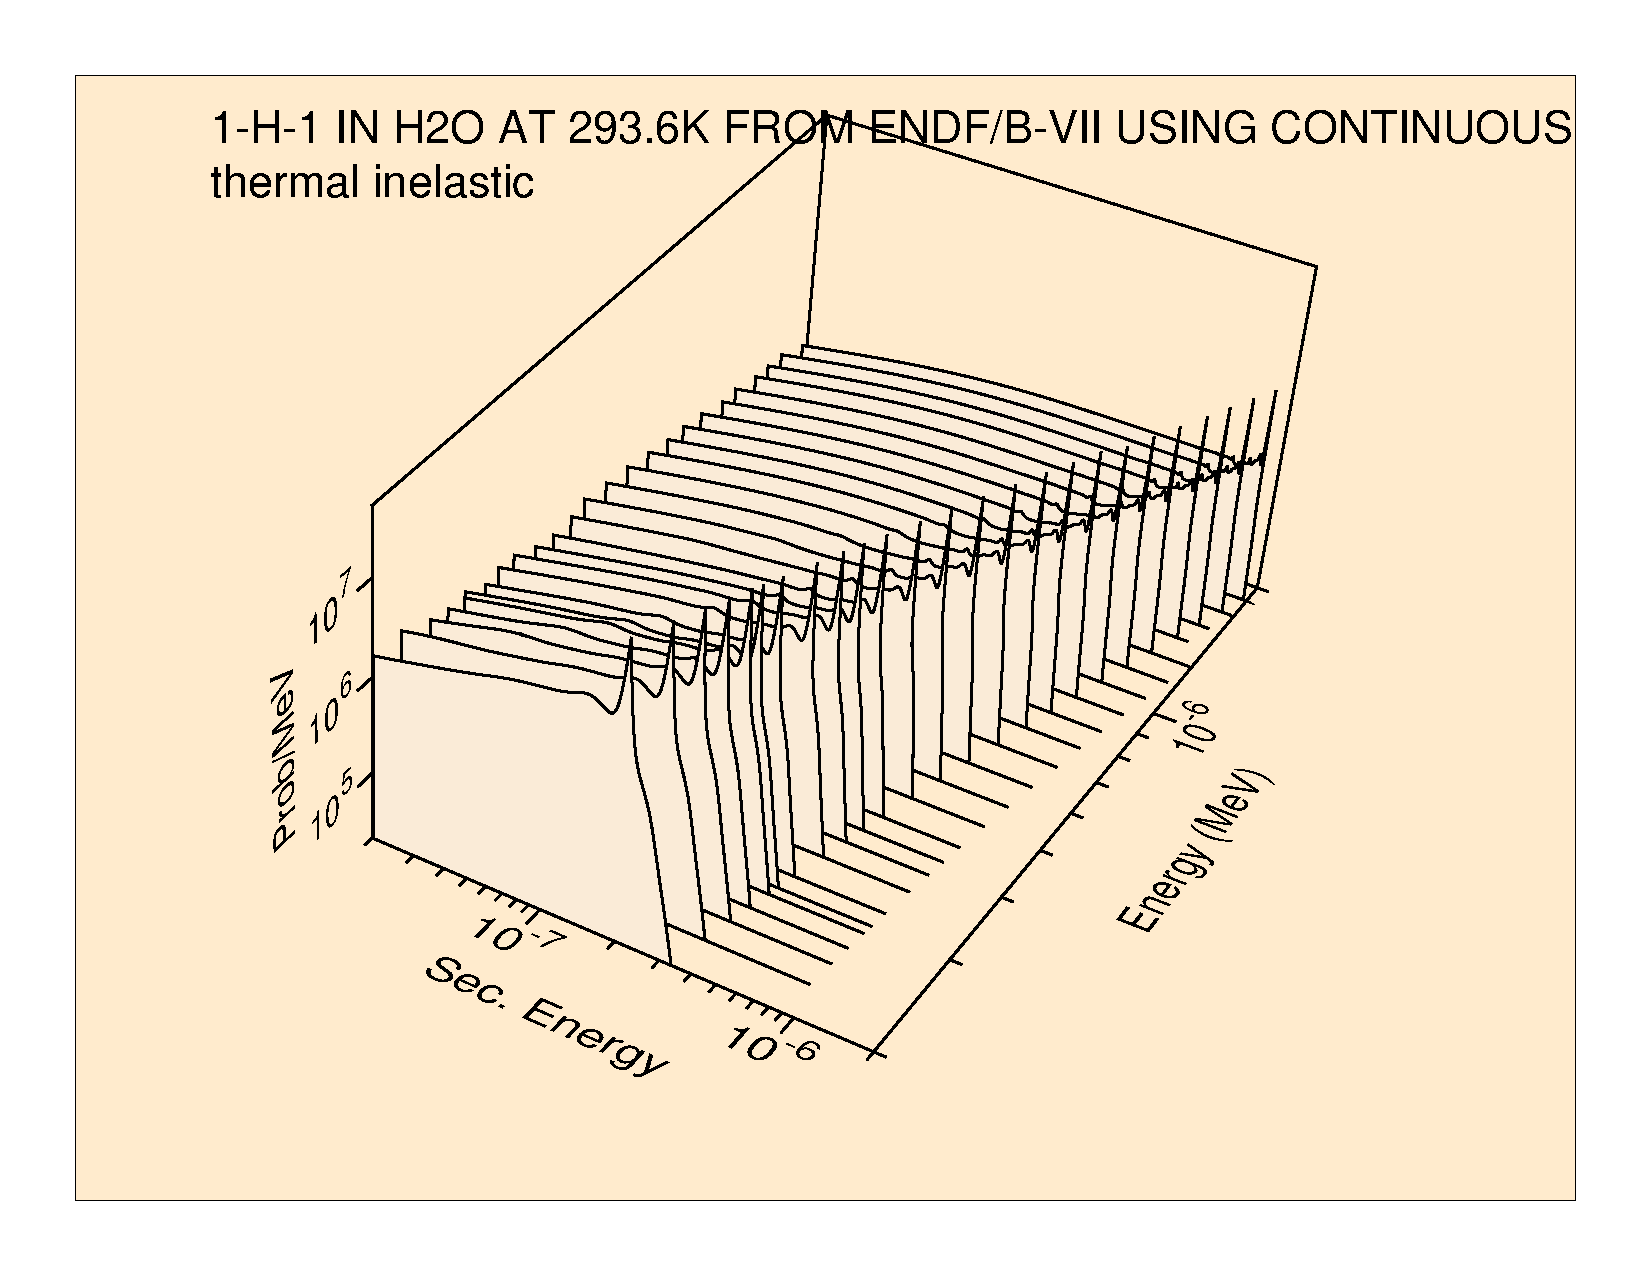
\includegraphics[keepaspectratio, height=3.5in, angle=0]{figs/thermr5ack}
\caption[Incoherent inelastic distribution for H-H$_2$O (expanded view)]
 {Expanded view of the high-energy region for the incoherent inelastic
 distribution of hydrogen bound in water.  Note the sharp quasi-elastic
 peak at $E{=}E'$.}
\label{water}
\end{figure}

A calculation of both free and graphite cross sections for ENDF/B-VII
carbon would go as follows:

\small
\begin{ccode}

 reconr
 20 22 / tape20 is carbon
 /
 600 1/
 .001/
 '6-C-nat from ENDF/B-VII'/
 0/
 broadr
 20 22 23/
 600 1/
 .001/
 293.6/
 0/
 thermr
 0 23 24/
 0 600 8 1 2 0 0 1 221 0/
 293.6/
 .005 5/
 thermr
 26 24 25 / tape 26 is ENDF/B-VII graphite
 31 600 8 1 2 1 0 1 229 0/
 293.6/
 .005 5/
 stop

\end{ccode}
\normalsize

\noindent
First, ENDF/B-VII carbon must be mounted on unit 20.  At LANL
this is done by copying it to a file named \cword{tape20} in the
user's local file space.  Similarly,  ENDF/B-VII graphite must be copied
to \cword{tape26}.  Next, \hyperlink{sRECONRhy}{RECONR} is run
to linearize the evaluation, and \hyperlink{sBROADRhy}{BROADR}
is run to prepare 293.6K cross sections.  The first THERMR
run is for free-gas scattering (\cword{mtref}=221), and the second run
is for carbon bound in graphite (\cword{mtref}=229).  Note that
\cword{natom} is now 1, and that 8 discrete angles were requested
in both cases.   For graphite, \cword{icoh} is set to 1 in order to
request the calculation of coherent elastic scattering like that shown
in Fig.~\ref{cohfig}.  The coherent results will use MF=3 and MT=230.
Distributions will be calculated to 0.5\% accuracy for energies up
to 5 eV.  The final PENDF file will be \cword{tape25}.

\subsection{Error Messages}
\label{ssTHERMR_msg}

\begin{description}
\begin{singlespace}

\item[\cword{error in thermr***nin=0}] ~\par
  An input PENDF tape is required.

\item[\cword{error in thermr***mode conversion not allowed}] ~\par
  \cword{nin} and \cword{nout} must both be binary or both be coded.

\item[\cword{error in thermr***illegal reference mt}] ~\par
  Restricted to MT=221--250.  User's should note that Card 2 has an
additional input parameter, \cword{iform}, beginning with
NJOY2012.  Unmodified NJOY99 input decks will produce this error message.

\item[\cword{error in thermr***desired material not on pendf tape}] ~\par
  Check input instructions against contents of thermal tape.

\item[\cword{error in thermr***desired temperature not on tape}] ~\par
  Check input instructions against contents of thermal tape.

\item[\cword{error in rdelas***too much elastic data}] ~\par
  There is not enough space in the allocatable array \cword{a}.
  See \cword{na}=10000.

\item[\cword{error in rdelas***desired temp not found}] ~\par
  The temperatures requested in THERMR must be the same as
  the temperatures on the input PENDF tape.

\item[\cword{error in coh***too many legendre orders}] ~\par
  The code currently computes only P$_0$, but \cword{nl}=1
  in \cword{coh} can be changed if desired.  Code is currently limited
  to 6 (P$_5$).  If more coefficients are desired, increase \cword{nlmax}
  and the dimensions of the variables \cword{s}, \cword{ej}, and \cword{ex}
  in \cword{coh}, \cword{calcem}, and \cword{tpend}.

\item[\cword{error in sigcoh***storage exceeded}] ~\par
  Not enough room for lattice factors.  Increase \cword{nw} which is
  currently 10000.

\item[\cword{error in sigcoh***illegal lat}] ~\par
  Only three lattices are coded so far.  To add others, insert the
  constants in \cword{sigcoh} and form factor formulas in \cword{form}.

\item[\cword{error in iel***bad temperature for debye-waller factor}] ~\par
  Shouldn't occur unless new materials are added incorrectly.

\item[\cword{error in iel***unknown material identifier}] ~\par
  Only three options are coded so far.  To add others, insert data
  statements for the Debye-Waller integrals and values for the
  bound cross sections.

\item[\cword{error in calcem***nl too large for binning}] ~\par
  Increase the value of the parameter \cword{nlmax} which is currently 33.

\item[\cword{error in calcem***storage exceeded}] ~\par
  There is not enough space in the global scratch array. Increase
  \cword{nwscr}, which is currently 99000, in \cword{thermr}.

\item[\cword{error in calcem***desired temperature not found}] ~\par
  Any temperature requested in THERMR must be on the input
  PENDF tape.

\item[\cword{error in calcem***bad temperature for teff}] ~\par
\item[\cword{error in calcem***bad temperature for teff2}] ~\par
  Data for effective temperatures use a temperature grid that
  is not consistent with the $S(\alpha,\beta)$ data.

\item[\cword{error in calcem***isabt=1 pendf tape found}] ~\par
  THERMR cannot process this format.

\item[\cword{error in calcem***only 2 sct atoms allowed}] ~\par
  For mixed moderators, such as BeO and Benzine, the SCT contribution
  from each atom must be included.  The code only allows for 2.

\item[\cword{error in calcem***too many angles}] ~\par
  For $E$-$\mu$-$E'$ ordering, there are more than \cword{mumax}=300
  angles being generated.

\item[\cword{error in sig***illegal option}] ~\par
 Only tabulated $S(\alpha,\beta)$ and free gas are coded at this time.

\item[\cword{error in sigl***no legal solution}]
\item[\cword{message from sigl---disc=-ffff, set to abs value....}]
\item[\cword{error in sigl***no legal solution (quadratic path)}] ~\par
  The code has trouble solving the equation for the boundary of a bin.

\item[\cword{error in tpend***storage exceeded}] ~\par
  Increase \cword{nwscr} in \cword{thermr}.

\item[\cword{error in tpend***cross section = 0}] ~\par
  Thermal cross section of zero cannot be used to normalize
  the distribution.

\end{singlespace}
\end{description}

\subsection{Input/Output Units}
\label{ssTHERMR_IOunits}

The following logical units are used.

\begin{list}{}{\leftmargin=.75in\labelsep=.25in\labelwidth=.5in}
\begin{singlespace}

\item[10/11] \cword{iold/inew} in \cword{thermr}.  Also used in
   \cword{coh}, \cword{calcem}, and \cword{tpend}.  Used for the
   \cword{loada/finda} scratch file that saves the energy grid
   and reaction cross sections.
\item[12]  \cword{nscr} in \cword{thermr}.  Also used in \cword{calcem}
   and \cword{tpend}.  Contains the scattering matrix before normalization.
\item[13]  \cword{nscr2} in \cword{thermr} and \cword{tpend}.  Contains
   data from \cword{nin} that are to be simply copied to \cword{nout}.
\item[20-99]  User's choice for \cword{nendf}, \cword{nin}, \cword{nout},
   and \cword{nread} (\cword{iinc}=2 only) to link with other modules.
   No mode conversion between \cword{nin} and \cword{nout} allowed.

\end{singlespace}
\end{list}

Units 10 and 11 are always binary.  Units 12 and 13 have the same mode
as \cword{nin} and \cword{nout}.  The user can choose the modes for
\cword{nendf}, \cword{nin}, \cword{nout}, except \cword{nin} and
\cword{nout} must have the same mode.

\subsection{Storage Allocation}
\label{ssTHERMR_storage}

The storage allocated in THERMR is for the \cword{loada/finda}
buffers and a scratch array.   The value of \cword{nbuf} my be changed
at will; larger values increase I/O efficiency.  The variable \cword{nwscr}
controls the maximum size of the TAB1 records of $\sigma(E\rightarrow E')$
versus $E'$ for incoherent scattering.  Hence it interacts with \cword{tol}.
The linearization stack (\cword{stk}) in \cword{coh} is controlled by
\cword{imax} and the number of Legendre components requested (always 1
in the standard version).  The current value of \cword{imax} (20) is
sufficient to divide each panel into parts as small as one-millionth
of the panel size.  The length of the list of lattice factors (\cword{fl})
in \cword{sigcoh} is controlled by the size of the ENDF/B File 7, and
\cword{nw}=10000 must be big enough for the problem.

\cleardoublepage

